% !TeX root = ../../main.tex
% ------------------------------------------------------------------
%  4.3 Data center primario y secundario: encabezado y 4.3.1, el primario.
%
% ------------------------------------------------------------------

\chapter{Data center}
\label{cap:4-3-data-center}

La estrategia de centros de datos distribuye la operación productiva entre la región primaria AWS sa-east-1 y la sala técnica secundaria del CD Talca. El dominio de nube se recupera en us-east-1; ante la pérdida de la sala de Talca, su WMS se levanta en la plataforma de nube de la región activa sobre la copia en Aurora. Concepción y las tres plataformas de cross-docking son sitios operacionales autónomos y publican sus eventos para la consolidación central.

La arquitectura fija RTO $\leq$ 4 h, RPO $\leq$ 15 min y disponibilidad mensual de 99,95 \% por componente de infraestructura, con un compromiso de $\geq$ 99,9 \% para la transacción crítica de extremo a extremo. Esta sección concreta los emplazamientos, servicios y conexiones descritos en 4.2; el equipamiento y los servicios contratados se detallan en el Formulario T-11, entregado como archivo propio.


\section{Especificaciones Data Center Primaria}
\label{sec:d-especificaciones-del-sitio-principal-on-}

El Data Center Primario concentra la operación productiva de la solución en dos dominios que se exigen mutuamente por el carácter híbrido obligatorio del despliegue: la región primaria de la nube en sa-east-1, ubicada en São Paulo, Brasil, y la sala técnica secundaria on-premise del centro de distribución de Talca, tipología que fija el propio caso. Ambos dominios se especifican bajo el mismo criterio: un centro de datos comprende no solo los servidores, sino también las condiciones que sostienen la operación sin interrupción: energía acondicionada, clima controlado, conectividad, seguridad física y monitoreo permanente con procedimiento escrito.

Esta sección declara, para cada dominio, el proveedor, la región y las zonas de disponibilidad, los servicios contratados y el sitio on-premise. También fija los objetivos de continuidad verificables que los gobiernan: disponibilidad de infraestructura de 99,95 \% mensual por componente y, para los servicios críticos, RTO $\leq$ 4 h y RPO $\leq$ 15 min. Sobre estos objetivos se sostiene el compromiso contractual penalizable de $\geq$ 99,9 \% mensual de la transacción de negocio de extremo a extremo. El desglose servicio por servicio y componente por componente se entrega en el Formulario T-11.

\subsection{Proveedor}

Para la nube en Amazon Web Services todos los servicios se contratan en cuentas del CLIENTE, que son organizadas bajo AWS Control Tower con una cuenta por ambiente de modo que la propiedad de los datos y de la infraestructura es del CLIENTE desde el primer día. Los criterios con que se eligieron esos servicios se explican en el apartado~\ref{sec:servicios-nube}. AWS satisface el requisito de presencia de región o zona en Chile o en Sudamérica con la región primaria sa-east-1. El cumplimiento de los estándares y marcos de referencia del Artículo 4.3 de las Bases Administrativas (art. 4.3, p. 5) entre ellos ISO/IEC 27017 (nube) e ISO/IEC 27018 (datos personales en nube) se acredita en la fila 5.23 de la matriz de controles del Anexo 4-R, que responde a RT-11.06 (Bases Técnicas Transversales, cap. 11, p. 23), y no se repite en esta sección.

En el dominio On-premise del CD de Talca, el caso exige cómputo, almacenamiento y procesamiento en las instalaciones del CLIENTE para sostener recepción, preparación y despacho durante un corte de enlace; ello obliga a la modalidad híbrida. Ese alcance requiere cómputo local para la continuidad de un sitio operacional sin albergar el núcleo. Por ello, el sitio adopta la tipología de \textbf{sala técnica secundaria o de sitio} del numeral 6.1 de las Bases Técnicas Transversales (cap. 6, p. 14), con disponibilidad de infraestructura de 99,95 \% y dimensionamiento proporcional al equipamiento real.

\subsection{Región y zonas de disponibilidad}

La región primaria de la nube es sa-east-1, ubicada en São Paulo, Brasil. Todo componente con requisito de alta disponibilidad se despliega en al menos dos zonas de disponibilidad; no se acepta un diseño en una sola zona. Aurora PostgreSQL tiene el escritor en sa-east-1a y un lector promovible en sa-east-1b. ECS Fargate, ElastiCache Redis, el balanceador de aplicación y el NAT Gateway operan entre esas mismas dos zonas con conmutación automática; DynamoDB opera Multi-AZ de forma nativa y transparente. El único componente con escritor único es la base de datos, que conmuta de forma automática entre las zonas. Este diseño sostiene el compromiso de extremo a extremo de $\geq$ 99,9 \% mensual de la transacción crítica y la conmutación se verifica en las pruebas de resiliencia por inyección de fallas de la arquitectura de despliegue.

\subsection{Servicios contratados en la región primaria}

Los servicios contratados en la región primaria son los que agrupa por función la Tabla~\ref{tab:servicios-nube} del apartado~\ref{sec:servicios-nube}. En esta región se concentran la operación productiva, la analítica y los servicios de detección, cumplimiento y gobierno; todos son servicios administrados, de modo que la solución no opera servidores en la nube.

\subsection{Sitio on-premise: CD Talca (sala técnica secundaria)}

El caso fija para el CD de Talca una sala técnica secundaria ``dimensionada para sostener recepción, preparación y despacho durante un corte'', y advierte que la sala actual de 25 m\textsuperscript{2} no cumple el Capítulo 6 de las Bases Técnicas Transversales (RT-06.01 del caso; Bases Técnicas del caso, cap. 15, p. 26). Conforme a la tipología del numeral 6.1 de las Bases Técnicas Transversales (cap. 6, p. 14), no se aplica íntegramente a este sitio el conjunto de exigencias de una sala técnica principal, sino el subconjunto dimensionado al sitio: energía, climatización, control de acceso, detección de incendio y monitoreo. El numeral 6.1 de las Bases Técnicas Transversales (cap. 6, p. 14) exige declarar la tipología y justificar el dimensionamiento, y advierte que ``sobredimensionar el recinto es tan penalizado como subdimensionarlo: ambos revelan que el cálculo de capacidad no se hizo''. El equipamiento real que la sala debe alojar y los cálculos eléctrico y térmico desarrollados a continuación determinan su superficie proyectada; la Figura~\ref{fig:recinto-talca} muestra su distribución interna por zonas y líneas de acceso.

La sala aloja el siguiente equipamiento:

\begin{itemize}
  \item El núcleo del componente on-premise, con el motor WMS y el borde operacional del CD sobre un clúster virtualizado de tres nodos con redundancia N+1, que tolera la pérdida de cualquier nodo manteniendo quórum.
  \item Una NAS local con el respaldo de recuperación rápida.
  \item Los dos firewalls de la frontera del sitio.
  \item El servidor del ERP de 2017 del CLIENTE, trasladado desde la sala actual.
\end{itemize}

La sala actual de 25 m\textsuperscript{2} del edificio de oficinas aloja hoy el servidor del ERP de 2017. Ese servidor se traslada sin cambios de software al rack R01 de la sala nueva, durante la Etapa 1, después del hito H3 y antes de la marcha blanca de Talca. El traslado ocurre en una ventana dominical, después de un respaldo completo verificado. Así, el ERP que emite las guías queda con UPS en N+1, generador de 24 horas, climatización redundante y control de acceso. La sala actual queda sin servidores y se libera para otro uso del CLIENTE (Bases Técnicas del caso, cap. 17, p. 33). Si el servidor tiene una sola fuente, se conecta a los circuitos A y B mediante un conmutador de transferencia de rack (RT-08.04; Bases Técnicas Transversales, cap. 8, p. 18).

El listado completo de componentes de sala (UPS, generador, climatización, seguridad física, extinción, cableado y gabinetes) y del equipamiento de cómputo y red que alojan los gabinetes se entrega en el Formulario T-11. La ocupación por rack y el margen de crecimiento se declaran en la Figura~\ref{fig:racks-talca}.

Para la disponibilidad y la redundancia la disponibilidad de infraestructura comprometida es del 99,95 \% mensual por componente en energía del recinto, climatización, red y comunicaciones, servidores y cómputo, y motor de base de datos. Además se sostiene con redundancia N+1 en energía y climatización, con generación autónoma y con monitoreo continuo con alertamiento. No se invoca una clasificación de instalación de terceros (ejemplo un nivel TIER certificado), por lo que los niveles de disponibilidad de infraestructura del numeral 7.2 de las Bases Técnicas Transversales (cap. 7, p. 17) son un medio, no un fin y el compromiso que se mide y se penaliza es el de la transacción de negocio de extremo a extremo.

La Figura~\ref{fig:cd-talca} muestra cómo se conecta el equipamiento de la sala con la bodega, la cadena de frío y el ERP.

\begin{figure}[htbp]
  \centering
  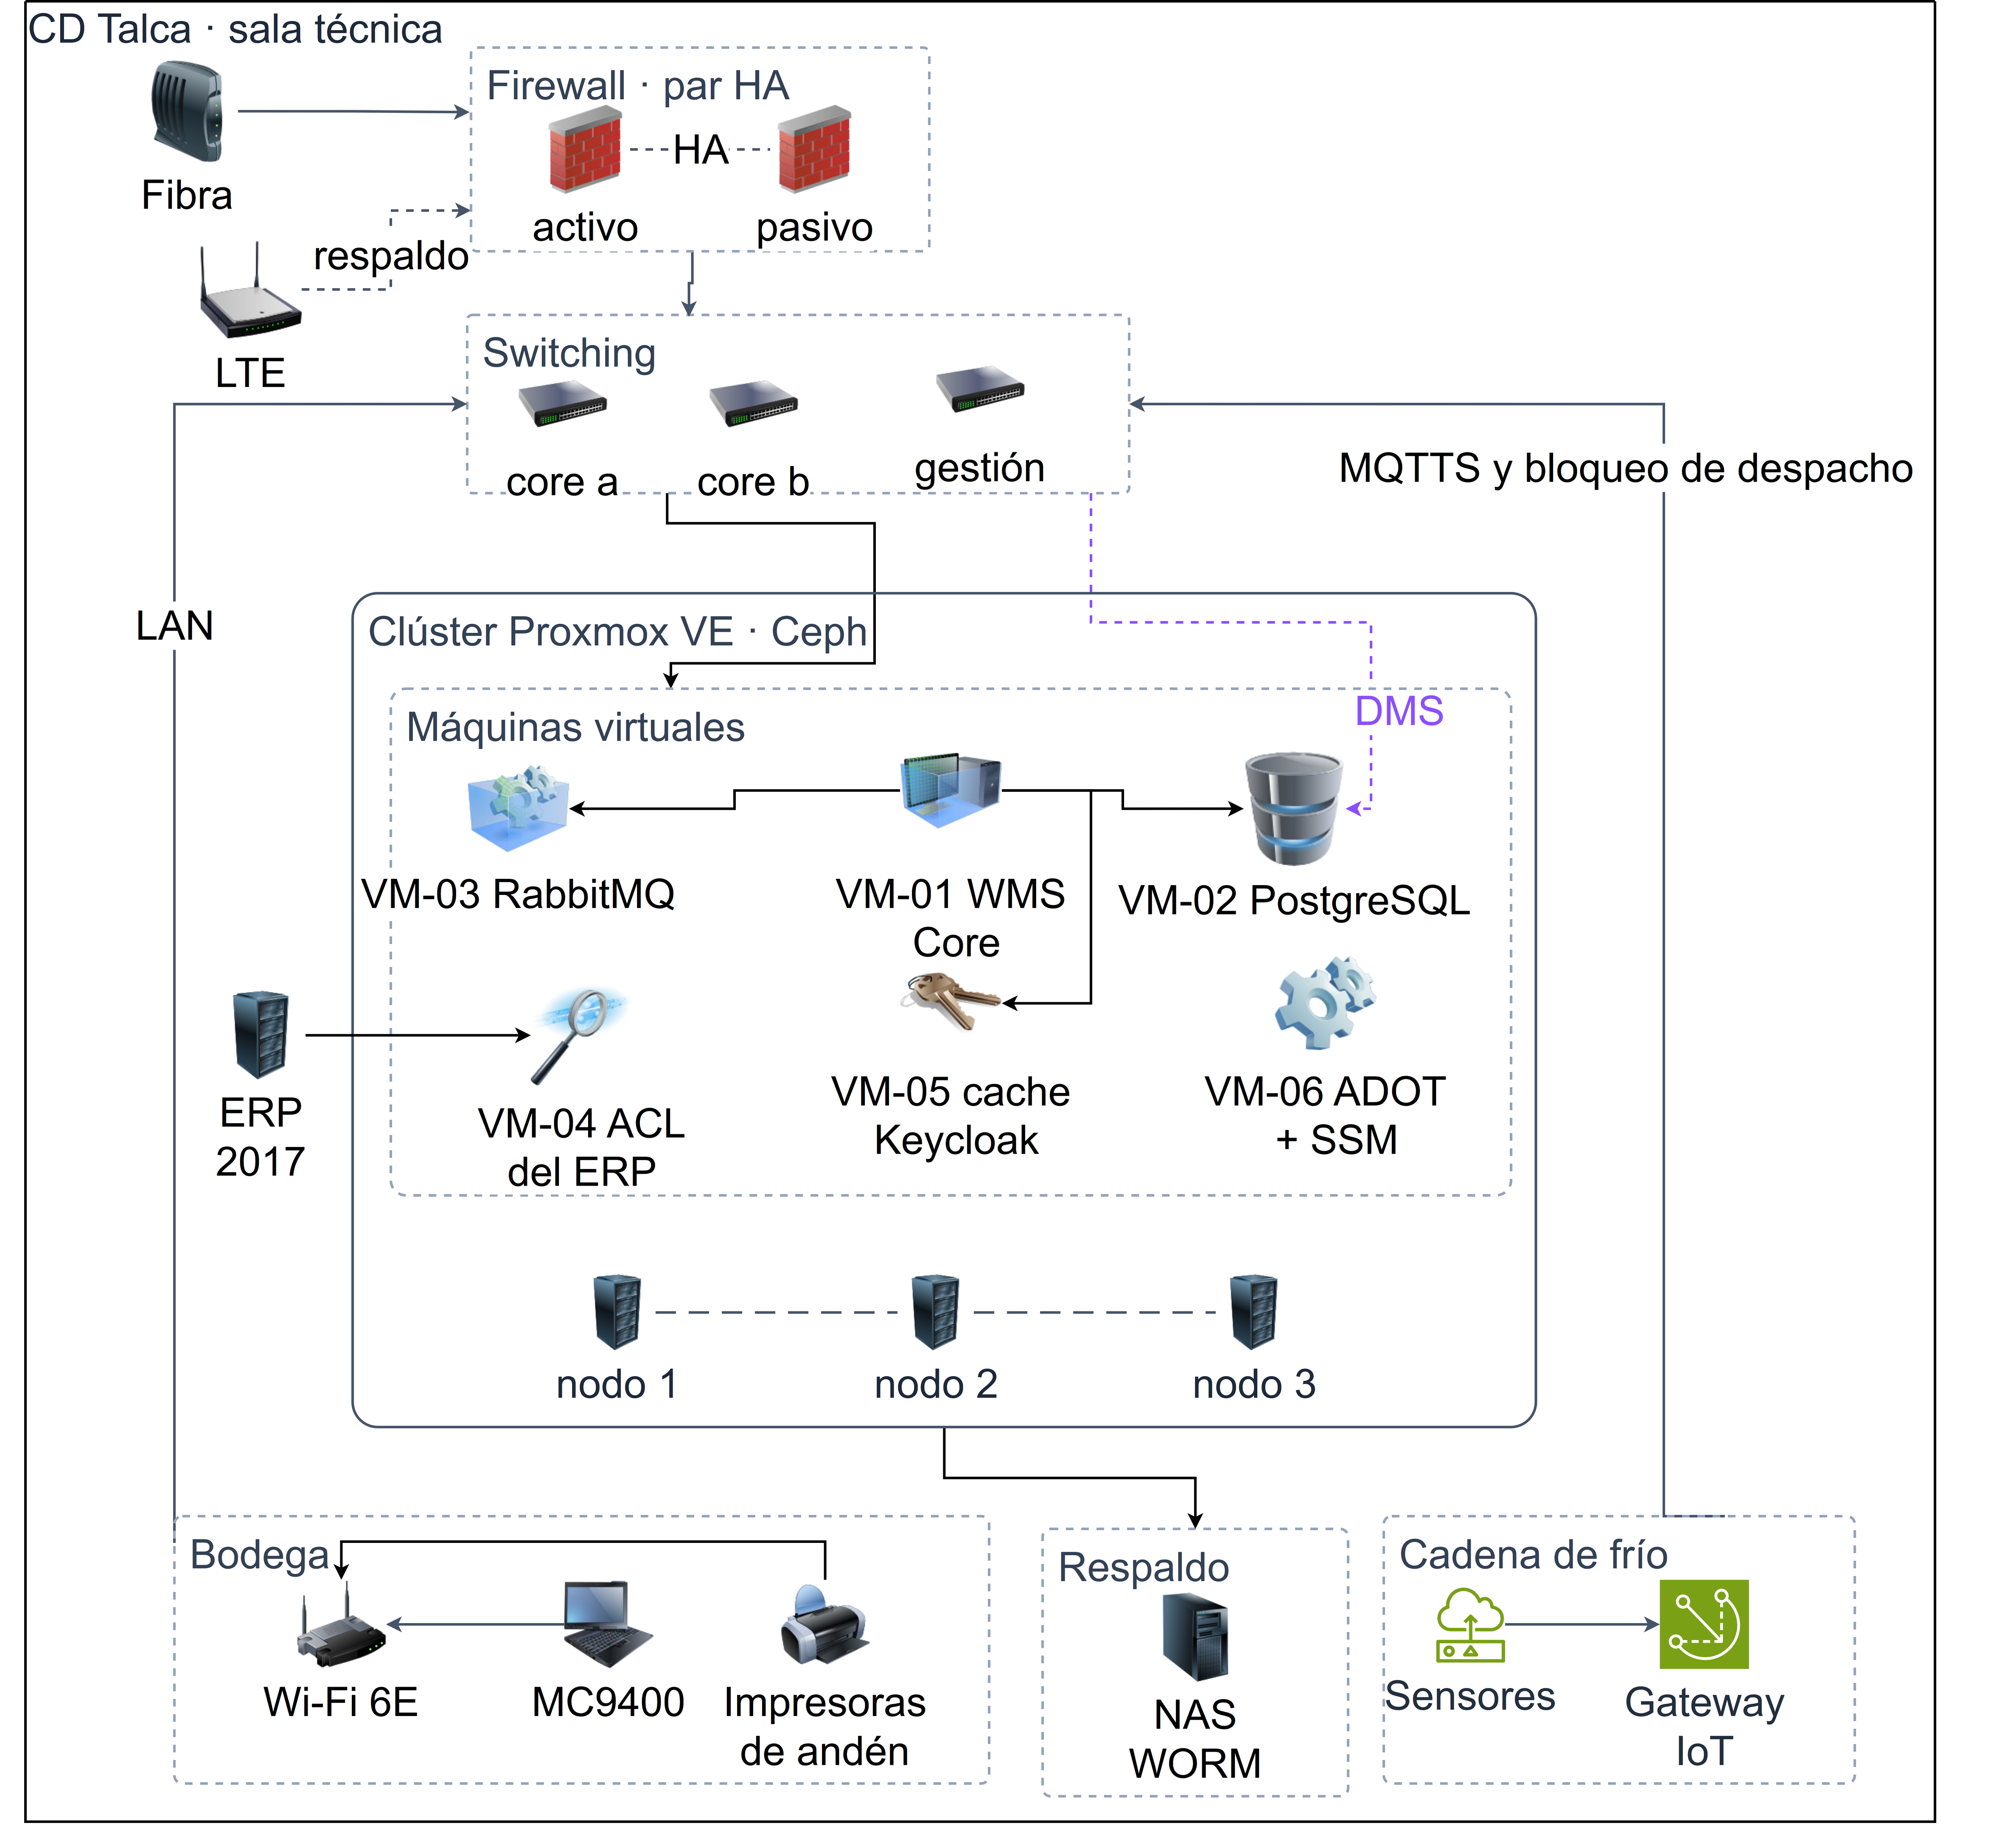
\includegraphics[width=\linewidth]{figuras/centros_de_datos/Arquitectura_Fisica_CD_Talca.png}
  \caption{Arquitectura física del sitio on-premise del CD Talca}
  \label{fig:cd-talca}
  \fuentefigura
\end{figure}
\FloatBarrier

La fibra D-03 es el enlace principal, LTE D-04 el segundo camino y Starlink D-06 el tercero en espera caliente; los tres llegan al par de firewalls, uno activo y otro pasivo. Starlink permanece encendido, con el túnel IPsec establecido y BGP con menor preferencia, y toma el tráfico solo si fallan fibra y LTE. En ese caso, la calidad de servicio prioriza DMS y WAL de Talca, la salida del broker y el outbox, las guías hacia el ERP y el SII, la identidad y la telemetría crítica. El terminal permanece encendido porque adquirir satélites y negociar el túnel durante una falla tardaría minutos; la tarifa plana no agrega costo por ello. Detrás, los dos switches de núcleo y el switch de gestión reparten la red hacia el clúster Proxmox VE con Ceph de tres nodos. El clúster aloja seis máquinas virtuales: VM-01 con el núcleo del WMS, VM-02 con PostgreSQL, VM-03 con RabbitMQ, VM-04 con la capa anticorrupción y los dos procesos de \texttt{erp-sync} que conversan con el ERP de 2017, VM-05 con la caché de Keycloak y VM-06 con el colector ADOT y el agente de Systems Manager. La línea punteada representa a AWS DMS, que lee los cambios de VM-02 por la VPN para replicarlos en Aurora. En la bodega, los terminales MC9400 y las impresoras de andén trabajan por Wi-Fi 6E contra el WMS; en la cadena de frío, los sensores entregan sus lecturas a los dos gateways IoT, que las publican por MQTTS y bloquean el despacho ante una excursión crítica y sostenida. El respaldo de recuperación rápida queda en la NAS WORM. La figura muestra que todo lo que la bodega necesita para recibir, preparar y despachar está dentro del sitio, y que la pérdida de un nodo no detiene la operación, porque sus máquinas virtuales se reinician en los otros dos.

La cadena eléctrica sigue esta secuencia: empalme $\rightarrow$ tablero general $\rightarrow$ transferencia automática $\rightarrow$ UPS $\rightarrow$ PDU del rack $\rightarrow$ fuente del equipo $\rightarrow$ servidor.

Esta cadena consta de UPS de doble conversión on-line en configuración N+1 con autonomía mínima de 30 minutos a plena carga y generación autónoma para un rango mínimo de 24 horas continuas, con estanque de combustible dimensionado y contrato de reabastecimiento declarado. La instalación eléctrica es independiente de la del resto del edificio y conforme a la normativa eléctrica chilena vigente, incluida la NCh Elec. 2777; se revisa y mide semestralmente, con informe entregable al CLIENTE, conforme a RT-06.10 (Bases Técnicas Transversales, cap. 6, p. 15).

Para el cálculo de carga eléctrica se usa una cota conservadora por equipo, según la Tabla~\ref{tab:4-3-1}: en los nodos, la suma de sus dos fuentes, y en los demás equipos, su potencia máxima de ficha. Para el servidor del ERP, cuya ficha no se conoce, se usa la misma cota de un nodo, que se confirma al medirlo en el levantamiento. El Formulario T-11 declara los mismos valores por equipo.

\begin{tablalafrox}{Carga eléctrica de TI proyectada del recinto}{tab:4-3-1}%
  {Y H{0.12} F{0.26} H{0.14}}%
  {\cab{Equipo} & \cab{Cantidad} & \cab{Potencia de placa por unidad} & \cab{Subtotal}}
  Nodo de cómputo del clúster (servidor rack 2U, un procesador) & 3 & 1.600 W (2 fuentes de 800 W) & 4.800 W \\
  NAS local & 1 & 400 W & 400 W \\
  Firewall del perímetro del sitio & 2 & 150 W & 300 W \\
  Conmutador de núcleo (switch core) & 2 & 150 W & 300 W \\
  Switch de gestión & 1 & 50 W & 50 W \\
  Servidor del ERP de 2017 (del CLIENTE, 2U) & 1 & 1.600 W (cota hasta medirlo) & 1.600 W \\
  \textbf{Carga TI base} & & & \textbf{7.450 W} \\
  Consola KVM (cubierta por el margen) & 1 & 50 W & Incluida en el margen \\
  Margen de crecimiento a tres años (20 \%) & & & + 1.490 W \\
  \textbf{Carga TI de diseño} & & & \textbf{8.940 W $\approx$ 8,9 kW} \\
\end{tablalafrox}

{\footnotesize Fuente: elaboración propia.\par}

El cálculo eléctrico sigue estos pasos:

\begin{enumerate}
  \item Potencia aparente y UPS: con factor de potencia 0,95, 8,9 kW $\div$ 0,95 $\approx$ 9,4 kVA; al 80 \% de utilización, 9,4 kVA $\div$ 0,8 $\approx$ 11,8 kVA. El UPS seleccionado es modular de 15 kVA, de doble conversión on-line, en configuración N+1 y con bypass de mantenimiento.
  \item PUE: la suma de 8,9 kW de carga TI, $\approx$ 2,7 kW de climatización de precisión, $\approx$ 0,4 kW de climatización de la sala de UPS, $\approx$ 0,6 kW de iluminación y apoyo y $\approx$ 0,78 kW de pérdidas del UPS es $\approx$ 13,4 kW; 13,4 $\div$ 8,9 $\approx$ 1,5. Los gateways IoT y sus fuentes agregan $\approx$ 0,1 kW al consumo del sitio, hasta $\approx$ 13,5 kW, pero quedan fuera del PUE de la sala. El PUE estimado y la carga declarada satisfacen RT-06.11 (Bases Técnicas Transversales, cap. 6, p. 15). El numerador se mide en el tablero del recinto y el denominador a la salida de las PDU, semestralmente y con informe entregable.
  \item Generador: la carga del sitio de $\approx$ 13,5 kW, con factor de potencia 0,8, requiere $\approx$ 13,5 $\div$ 0,8 $\approx$ 16,9 kVA. Se especifica un grupo electrógeno de 25 kVA, que deja la carga de diseño en el 68 \% de su capacidad, bajo el 80 \%, con estanque para 24 horas continuas y contrato de reabastecimiento.
\end{enumerate}

La climatización de precisión para la operación continua es redundante en configuración N+1 y controla la temperatura y la humedad relativa dentro de los rangos que recomienda el fabricante del equipamiento.

Para calcular la carga térmica, se considera que cada kW eléctrico consumido por el equipamiento se disipa físicamente como aproximadamente 1 kW de calor sensible ($\approx$ 3.412 BTU/h). Como el UPS está en su propia sala, la carga térmica de la sala de servidores corresponde a la carga TI de diseño, como resume la Tabla~\ref{tab:4-3-2}:

\begin{tablalafrox}{Carga térmica sensible proyectada del recinto}{tab:4-3-2}%
  {Y F{0.26}}%
  {\cab{Origen del calor} & \cab{Potencia equivalente}}
  Carga TI de diseño & 8.940 W \\
  \textbf{Carga térmica sensible de diseño} & \textbf{$\approx$ 8,9 kW} \\
\end{tablalafrox}

{\footnotesize Fuente: elaboración propia.\par}

Sobre esa carga se instalan dos unidades de climatización de precisión de 10 kW cada una, en configuración N+1; una sola cubre los 8,9 kW de diseño. La temperatura y la humedad relativa se controlan dentro de los rangos del fabricante del equipamiento. La sala de UPS y baterías dispone de climatización de confort propia de 3,5 kW ($\approx$ 12.000 BTU/h), que mantiene 20--25\,\textdegree{}C, y de ventilación; disipa las pérdidas del UPS ($\approx$ 0,78 kW) y el calor de carga de las baterías.

La consola KVM, con 50 W de potencia de placa, el conmutador de transferencia del ERP y los equipos terminales de acceso del operador (ONT de fibra, router LTE y terminal Starlink) quedan cubiertos por el margen de diseño del 20 \% de la Tabla~\ref{tab:4-3-1}, sin alterar el UPS de 15 kVA ni el generador de 25 kVA.

La protección contra incendios reúne estos elementos:

\begin{itemize}
  \item Detección temprana por aspiración de aire con tecnología láser, tipo AnaLASER.
  \item Extinción automática con agente limpio tipo FM-200 con aprobación UL e instalación conforme a norma NFPA, con botón de aborto.
  \item Sistema secundario de extintores portátiles habilitados con mantención y certificación vigentes.
\end{itemize}

El sistema de detección y extinción se integra al monitoreo en línea y notifica al NOC y a la contraparte del CLIENTE.

La Figura~\ref{fig:racks-talca} muestra cómo se reparte el equipamiento de cómputo y red en los dos racks de la sala.

\begin{figure}[htbp]
  \centering
  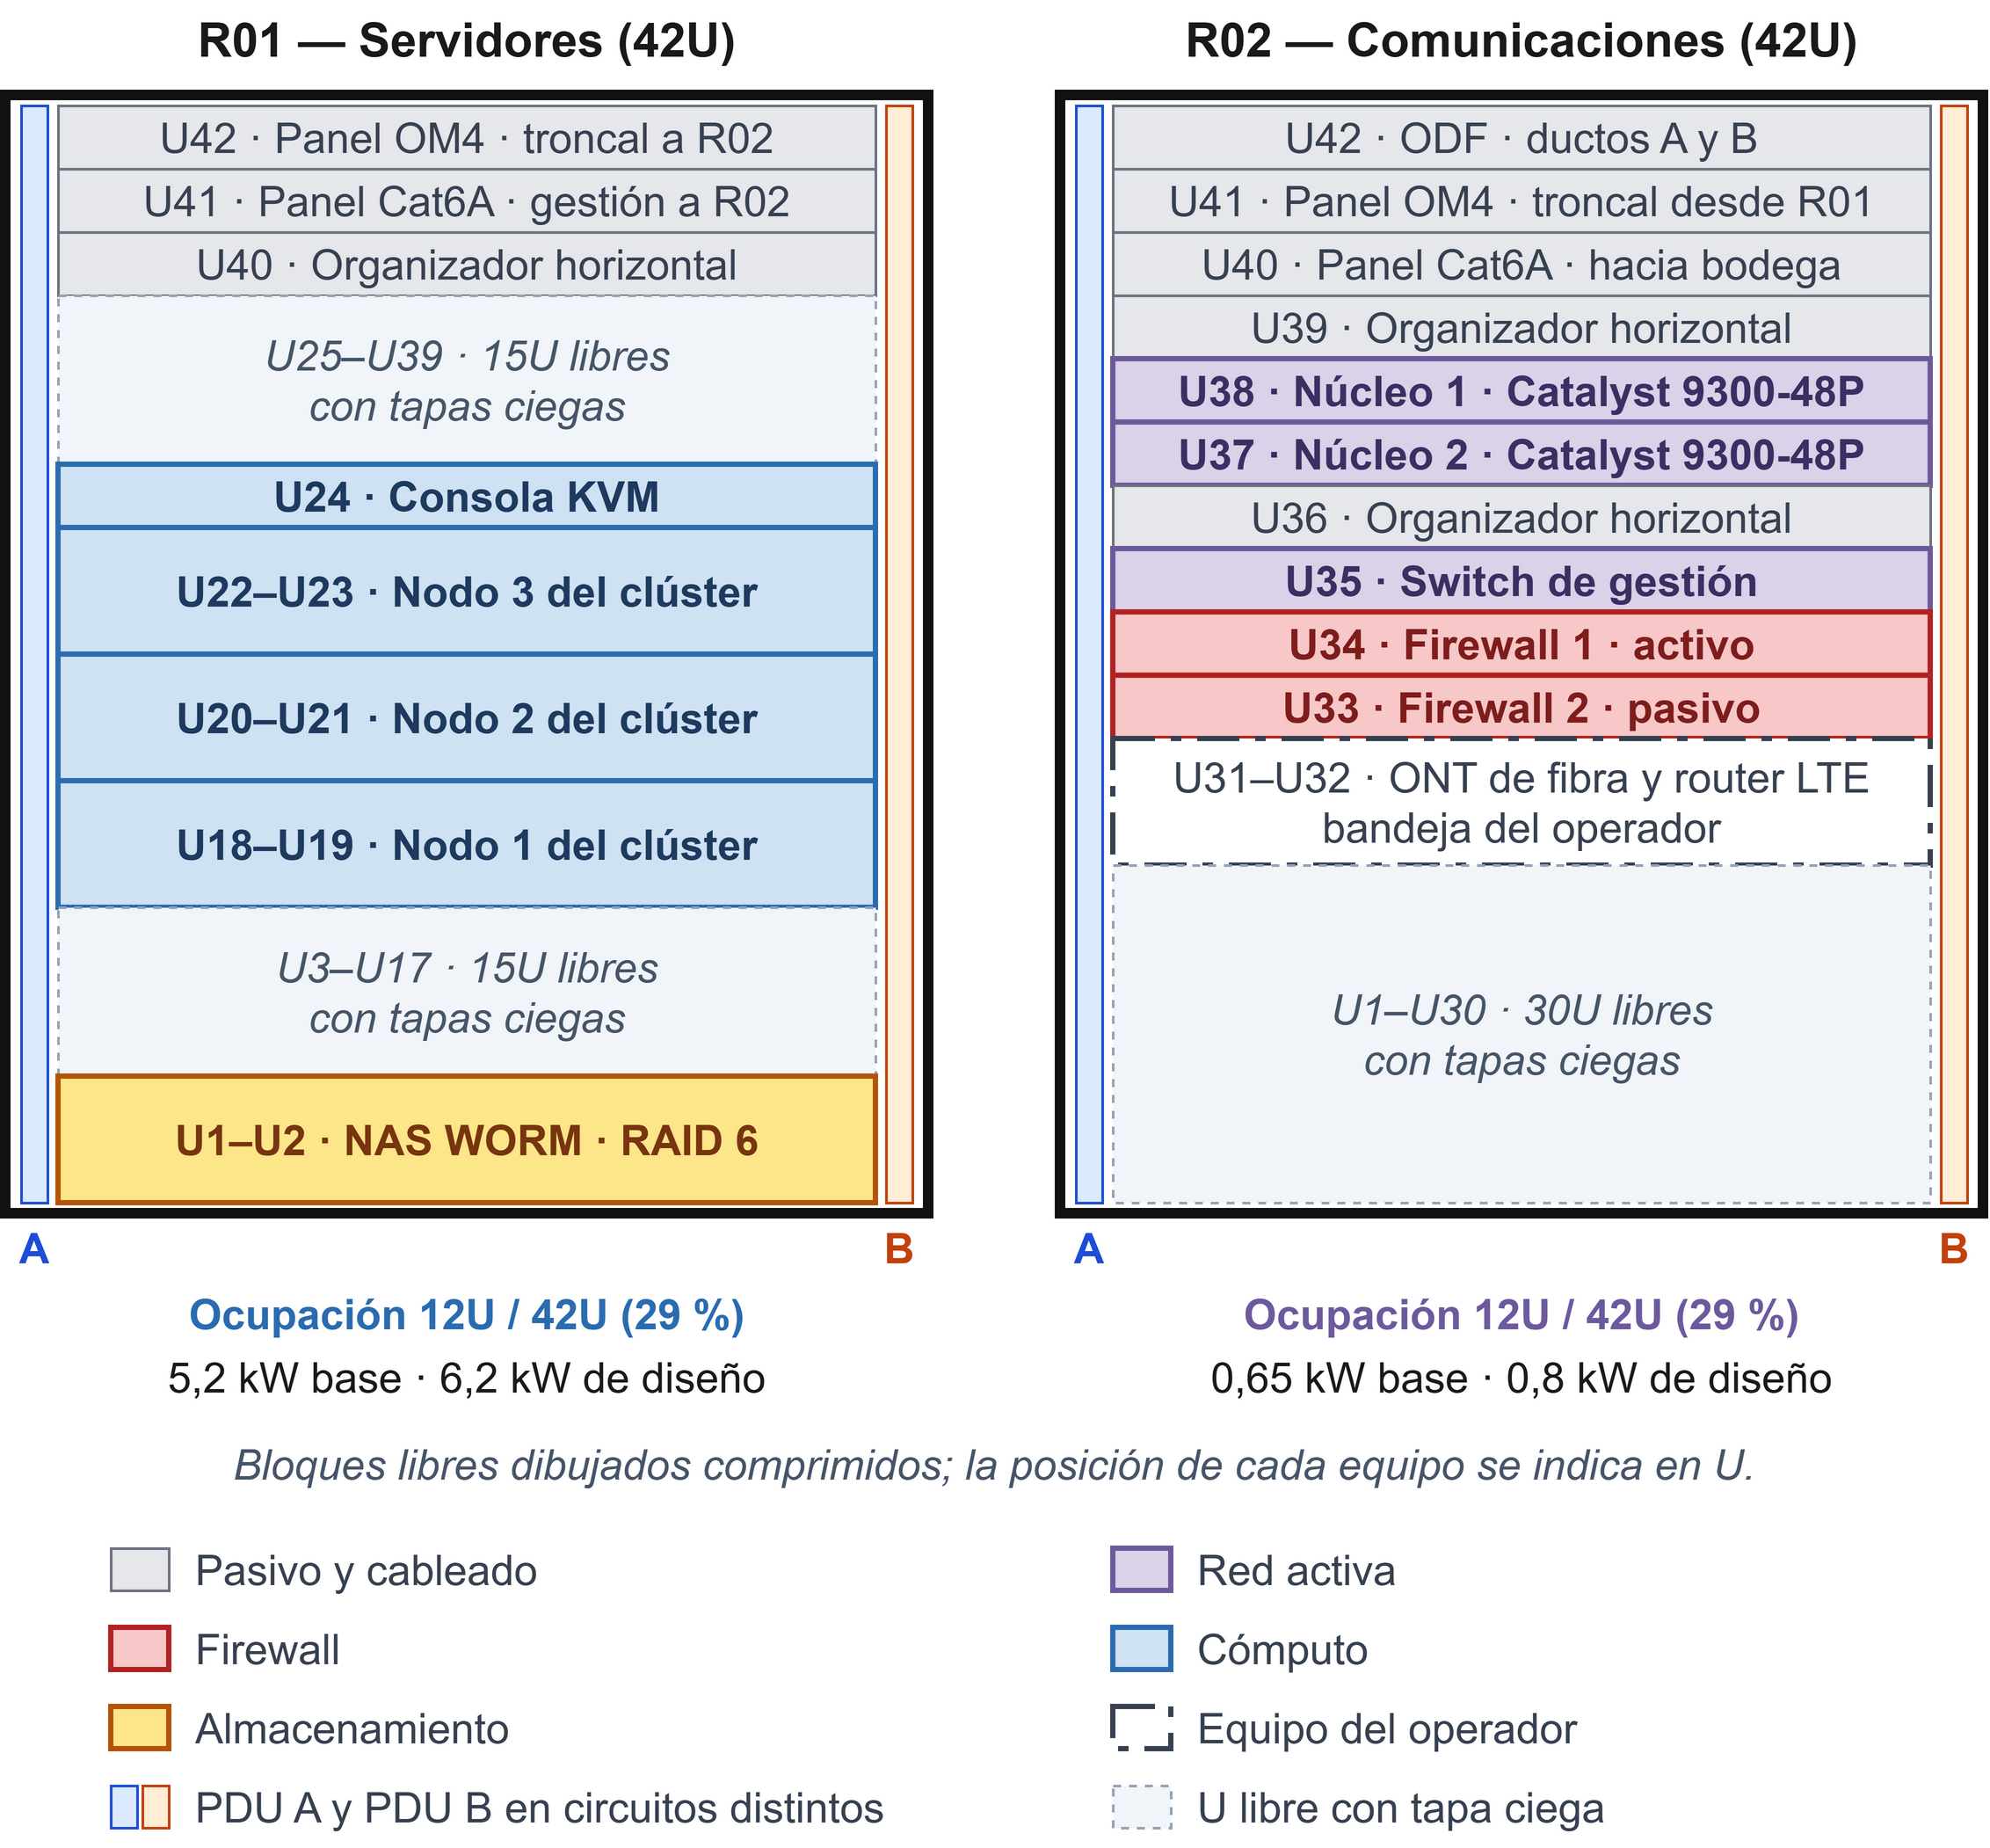
\includegraphics[width=\linewidth]{figuras/centros_de_datos/Racks_CD_Talca.png}
  \caption{Distribución de U y ocupación proyectada de los racks del CD Talca}
  \label{fig:racks-talca}
  \fuentefigura
\end{figure}
\FloatBarrier

El rack R01 aloja los tres nodos del clúster, de 2U cada uno, la consola KVM, la NAS WORM, el servidor del ERP de 2U y su conmutador de transferencia; el rack R02 aloja el ODF, los paneles, los dos switches de núcleo, el switch de gestión, el par de firewalls y la bandeja del operador con la ONT de fibra y el router LTE. R01 ocupa 15U de 42 (36\,\%) y R02, 12U (29\,\%). La carga de R01 es de 6,8 kW base y 8,2 kW de diseño, y la de R02, de 0,65 kW base y 0,8 kW de diseño; las cargas base suman los 7.450 W de la Tabla~\ref{tab:4-3-1}, y las de diseño, los 8,9 kW que resultan al agregar el margen de 20\,\%. La figura dibuja comprimidos los bloques libres e indica la posición de cada equipo en U. Los racks de servidores son independientes de los racks de equipos de comunicación. La ocupación proyectada reserva margen de crecimiento a tres años, coherente con el 20 \% de reserva de la carga eléctrica (Tabla~\ref{tab:4-3-1}), de modo que la ocupación declarada y su margen quedan fijados en la figura y en el Formulario T-11.

El control de acceso y la seguridad física del recinto comprenden:

\begin{itemize}
  \item Seguridad física y control de acceso biométrico basado principalmente en biometría facial con AFIS como respaldo.
  \item Registro de todo ingreso y egreso en una bitácora auditable con identificación, fecha, hora y motivo.
  \item Un espacio para atender a las personas en proceso de enrolamiento entre el acceso principal y el término del pasillo de la zona de control, además de una estación de enrolamiento fuera de las instalaciones del recinto técnico.
  \item Un acceso al término del pasillo que impide el paso de más de una persona a la vez, con nueva verificación de identidad previa al ingreso.
  \item Videovigilancia y monitoreo IP con imágenes en línea disponibles al menos los últimos 30 días y respaldo recuperable.
\end{itemize}

Las instalaciones sanitarias, las zonas de seguridad ante emergencia y las áreas exteriores existentes en el edificio del CLIENTE se utilizan, sin implementarlas nuevamente dentro del recinto. La bitácora auditable se conserva por un período de retención no inferior a cinco años, coherente con el piso de retención de la auditoría que fija RT-16.10 (Bases Técnicas Transversales, cap. 16, p. 29).

Los equipos de energía y climatización y los controles de acceso descritos se ordenan físicamente como muestra la Figura~\ref{fig:recinto-talca}, que distribuye el recinto por zonas y líneas de acceso.

\begin{figure}[htbp]
  \centering
  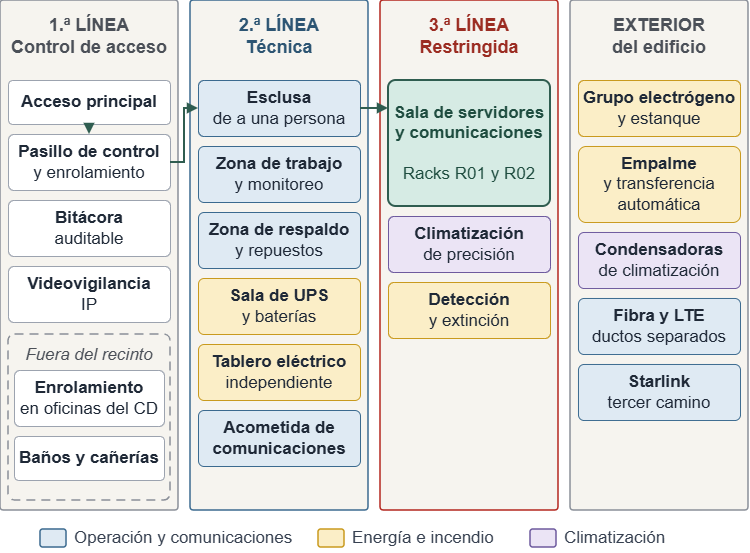
\includegraphics[width=\linewidth]{figuras/centros_de_datos/Recinto_CD_Talca.png}
  \caption{Distribución interna del recinto técnico del CD Talca por zonas y líneas de acceso}
  \label{fig:recinto-talca}
  \fuentefigura
\end{figure}
\FloatBarrier

La distribución ordena el recinto en profundidad progresiva. En el exterior quedan el grupo electrógeno con su estanque, el empalme con la transferencia automática entre red y generador, las condensadoras de la climatización y la llegada independiente de fibra, LTE y Starlink. La fibra y LTE ingresan al edificio por puntos separados y siguen ductos independientes hasta la sala, conforme a RT-06.32 (Bases Técnicas Transversales, cap. 6, p. 17); Starlink constituye el tercer camino. La línea técnica reúne la sala de UPS y baterías, el tablero eléctrico independiente del recinto y la acometida de comunicaciones, junto con la zona de trabajo y la zona de respaldo. La línea restringida contiene solo la sala de servidores y comunicaciones, con los racks R01 y R02, la climatización de precisión y la detección y extinción. El ingreso sigue un único recorrido: acceso principal, pasillo de control con espacio de enrolamiento, esclusa que admite una persona a la vez con nueva verificación y, recién entonces, la sala; la estación de enrolamiento y los baños quedan fuera del recinto. Los puestos de trabajo y el área de respaldo quedan en la línea técnica, separados de la sala de equipos, de modo que las labores habituales de operación no exigen ingresar a la línea restringida. La separación física de generadores y baterías respecto del área de servidores evita que una falla de energía o de clima contamine el cómputo, y deja al proveedor de fibra y al de climatización sin cruzar la última línea del recinto.

El sitio monitorea en línea la temperatura, la humedad y la presencia de agua, con alertamiento integrado a la plataforma de observabilidad. El estado de los puntos controlados del recinto converge en la plataforma de monitoreo, con destinatario, canal, tiempo de respuesta y procedimiento escrito. La observabilidad reutiliza el mecanismo del sitio on-premise hacia la nube que define la arquitectura de despliegue del apartado~\ref{sec:despliegue}. La convergencia en un solo tablero constituye la plataforma de observabilidad del sitio. No se declara una plataforma DCIM/BMS de terceros porque las Bases no la exigen y el monitoreo ambiental y de alertas se satisface con el monitoreo en línea y su alertamiento integrado.

El cómputo local corre sobre un clúster virtualizado de tres nodos N+1 con quórum real. Ceph distribuye tres réplicas sobre NVMe sin RAID y tolera la pérdida de un nodo; el respaldo local reside en el NAS D-05 con RAID 6. La selección se justifica en ADR-10 (Anexo 4-O). La instancia de escritura VM-02 se reinicia en otro nodo ante una falla.
